\section{Framework-Wide Design Elements}
\label{sec:fwdesign}

The following sections describes design choices that apply across the 
entire body of ESMF software.

\subsection{ESMF Base Object}

All ESMF objects are based on the object below.  Attributes
can be handled by generic routines, but it is expected that 
higher level objects will supply their own class specific
methods of the ones listed below.

\scalebox{0.70}{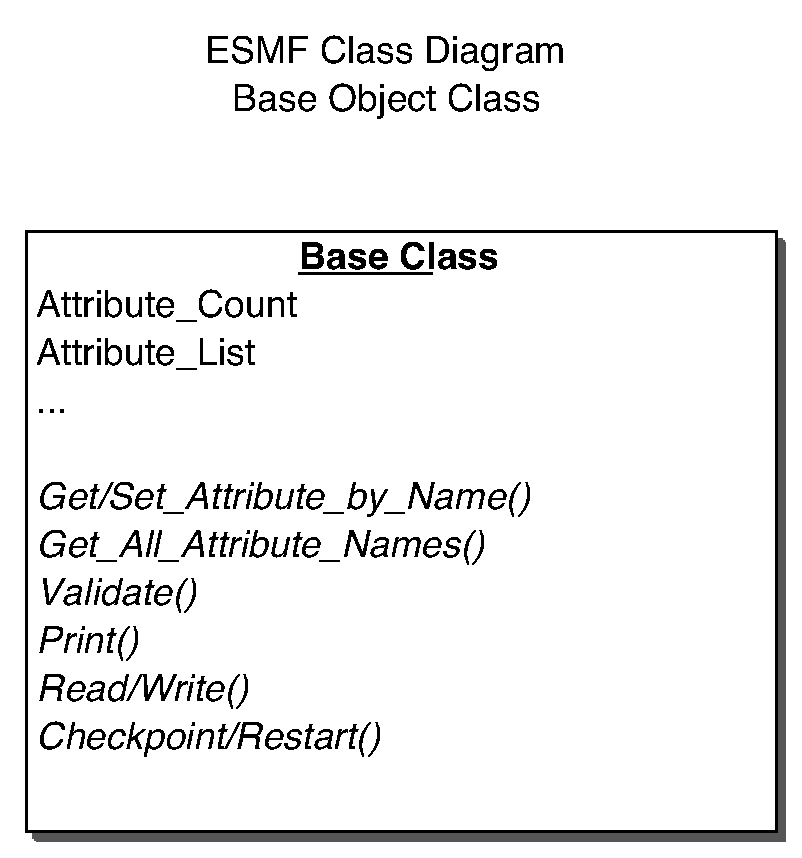
\includegraphics{ESMF_Base.eps}}

\subsubsection{Base (ESMF\_Base)}
\label{sec:Base} 
\begin{description}
\item [Description] The ESMF Base class is an abstraction of the private data and
methods common to all other object in the system.  Some methods and data can be
inherited direcly from the Base class; others are expected to be overloaded by
higher level objects.
\item [Function] The Base class methods which are expected to be overloaded by
more specialized objects include: Print, Validate, Read/Write, Checkpoint/Restart.
Methods which are inherited by all other classes include those which 
set and query object Attributes.
\end{description}








